\section{单因素完全随机实验设计}
\subsection{基本特点}

完全随机设计(completely randomized design)的假定是,由于被试是从总体中随机选取,处理也是随机分配给被试,那么被试间的差异也是随机、在统计上无差异的.



\begin{margintable}
	\centering
	\caption{单因素完全随机实验设计中被试的分配}
	\labtab{one_way_ANOVA_data}
	{
		\begin{tabular}{cccc}
			\toprule
			$a_1$ & $a_2$ & $a_3$ & $a_4$ \\
			\midrule
			$S_1$ & $S_2$ & $S_3$ & $S_4$ \\
			$S_5$ & $S_6$ & $S_7$ & $S_8$ \\
			$S_9$ & $S_{10}$ & $S_{11}$ & $S_{12}$ \\
			$S_{13}$ & $S_{14}$ & $S_{15}$ & $S_{16}$ \\
			\bottomrule
			% \addlinespace[1ex]
			% \multicolumn{6}{p{0.5\linewidth}}{\textit{Note.} Type III Sum of Squares} \\
		\end{tabular}
	}
\end{margintable}

单因素完全随机设计中分配被试的图解例子如\vreftab{one_way_ANOVA_data},
个因素$A$有4个水平,每个处理下有4个被试.完全随机设计是一种被试间设计,这意味着每一个被试只接受一种处理或处理的组合
\sidenote[*-5][]{处理的组合是多因素实验中会遇到的,后面遇到了再说}
,故对于本例而言需要16个被试.

对接下来要描述的模型的字母进行一下简要的说明:

(1)假设因素$A$有$p$个水平,用$\alpha _j$表示其第$j$个水平($1 \leq j \leq p$),也就是说$A$的水平分别是$\alpha _1,\cdots,\alpha _j,\cdots, \alpha _p$,

(2)$p$个处理下的被试数都相等,均为$n$个,用$i$表示每个处理下第$i$个被试($1 \leq i \leq n$)

(3)假设被试在没有施加处理的时候,无限次实验结果的平均数是$\mu$.该值是个理想值,其实意思是被试测量值在理论上的基线,不过这么说只是表达了概念.虽然说明了更加明确的定义不过可以充分的感受到,这个理论基线值是无法获得的,毕竟无限次是个极限,不是一个具体的数,所以$\mu$是个理论值.

(4)假设实验中的误差是$\varepsilon _{i\left(j\right)}$
\sidenote{注意误差的下标是带有括号的,这点以后再解释.}
,其平均数为0,方差为$\sigma _e^2$,我们进一步假设它服从正态分布

(4)观察值$Y_{ij}$指第$j$个处理水平下,第$i$个被试的观测值

后现的章节因素多了会加入一些新字母和下标,和上述符号已经没有本质区别,故以后我不打算再介绍新符号了.

\subsubsection{单因素完全随机实验设计模型}
\begin{definition}[单因素完全随机实验设计模型]
\labdef{one_way_random_model}

\begin{align*}
    Y_{ij}=\mu +\alpha _j+ & \varepsilon _{i\left( j \right)}\\
                           & \left( j=1,2,\cdots,p ; i=1,2,\cdots,n \right)
\end{align*}

其中:

{\renewcommand\arraystretch{1.25}
\begin{tabular}{lcl}
    $Y_{ij}$ & - & 被试$i$在处理水平$j$上的分数 \\
    $\mu$ & - & 总体平均数 \\
    $\alpha _j$ & - & 水平$j$的处理效应 \\
    $\varepsilon_{i \left( j \right)}$ & - & 误差效应 \\
\end{tabular}}

\end{definition}

\subsubsection{单因素随机区组实验设计检验的假说}
单因素完全随机设计的原假说是:多个处理水平上的总体平均数相等,即
\[  H_0: \mu _{.1}=\mu _{.2}=\cdots=\mu _{.p}  \]

或处理效应等于为0,即
\[  \alpha _j=0  \]







\subsection{实验设计与计算举例}

\subsubsection{研究的问题}
我想研究文章的生字密度对学生阅读理解的影响.我的假设是:阅读理解随着文章中生字密度的增加而下降。因此,该实验有一个自变量——生字密度,通过研究前人文献我感兴趣的是四种生字密度
(1)$5:1\left(a_1\right)$、
(2)$10:1\left(a_2\right)$、
(3)$15:1\left(a_3\right)$、
(4)$20:1\left(a_4\right)$
因变量是被试的阅读理解分数。实施实验时,我将32名被试随机分成四组,每组被试阅读一种生字密度的文章,并回答阅读理解测验中有关文章内容的问题。这是一个典型的单因素完全随机设计。虽然我不再检验实验中其他因素的影响,但实际上存在着诸多对因变量影响的无关变量,比如文章的长度、文章的主题熟悉性、文章类型等,还有被试的年龄、受教育程度、阅读能力等。这时,控制无关变量可做的工作之一是在选取四篇文章时,使它们在除生字密度以外的其他方面尽量匹配。

\subsubsection{新的计算模型的引入以及数据的计算}
我将引入一种新的计算模式,这种模式主要是为了手算.为了理解愿意,我们必须手算一次每种实验设计的简单数据,但是用统计教材上的算法根本无法实现一个较为精确的估算,其原因是,和方的计算公式选用:

$$
    SS =
        \sum\limits_{i=1}^{n}
        \left( 
            X_i -\bar{X} 
        \right)^2
$$

式子中$\bar{X}$很大可能是小数,且可能是循环小数,所以每次相减都会四舍五入,然后平方后进一步放大误差,这样算到最后误差不断累记.所以应当最后一步再做除法,把上面的式子改写一下:

\begin{align*}
SS  & = \sum\limits_{i=1}^n{\left( X_i-\bar{X} \right) ^2}
\\
    & =\sum\limits_{i=1}^n{\left( X_{i}^{2}+\underset{\text{常数}}{\underbrace{\bar{X}^2}}-\underset{\text{常数}}{\underbrace{2\bar{X}}}X_i \right)}
\\
    & =\sum\limits_{i=1}^n{X_{i}^{2}}+n\bar{X}^2-\underset{2n\bar{X}^2}{\underbrace{2\bar{X}\sum\limits_{i=1}^n{X_i}}}
\\
    & =\sum\limits_{i=1}^n{X_{i}^{2}}-n\left( \frac{\sum\limits_{i=1}^n{X_i}}{n} \right) ^2
\\
    &= \underset{\text{离散+集中+可能个体差异}}{\underbrace{\sum\limits_{i=1}^n{X_{i}^{2}}}}-\underset{\text{集中}}{\underbrace{\frac{\left( \sum\limits_{i=1}^n{X_i} \right) ^2}{n}}}
\end{align*}

这样除法只进行了一次(上式“集中”那里算了一次除法,产生误差),其余的都是乘法和加法.那么在方差分析中,大量求$SS$,用这样的方法就可以利于手算,以便更好了解方差分析原理.


\textbf{1.计算表}

\begin{margintable}
	\centering
	\caption{单因素完全随机实验的$AS$表}
	\labtab{one_way_ANOVA_AS_TAB}
	{
		\begin{tabular}{cccccc}
			\toprule
    			     & $a_1$ &  $a_2$ &  $a_3$ &  $a_4$ & \\
    			     \midrule
                              & \cellcolor[rgb]{ .949,  .949,  .949}3 & \cellcolor[rgb]{ .949,  .949,  .949}4 & \cellcolor[rgb]{ .949,  .949,  .949}8 & \cellcolor[rgb]{ .949,  .949,  .949}9 &  \\
                              & \cellcolor[rgb]{ .949,  .949,  .949}6 & \cellcolor[rgb]{ .949,  .949,  .949}6 & \cellcolor[rgb]{ .949,  .949,  .949}9 & \cellcolor[rgb]{ .949,  .949,  .949}8 &  \\
                              & \cellcolor[rgb]{ .949,  .949,  .949}4 & \cellcolor[rgb]{ .949,  .949,  .949}4 & \cellcolor[rgb]{ .949,  .949,  .949}8 & \cellcolor[rgb]{ .949,  .949,  .949}8 &  \\
                              & \cellcolor[rgb]{ .949,  .949,  .949}3 & \cellcolor[rgb]{ .949,  .949,  .949}2 & \cellcolor[rgb]{ .949,  .949,  .949}7 & \cellcolor[rgb]{ .949,  .949,  .949}7 &  \\
                              & \cellcolor[rgb]{ .949,  .949,  .949}5 & \cellcolor[rgb]{ .949,  .949,  .949}4 & \cellcolor[rgb]{ .949,  .949,  .949}5 & \cellcolor[rgb]{ .949,  .949,  .949}12 &  \\
                              & \cellcolor[rgb]{ .949,  .949,  .949}7 & \cellcolor[rgb]{ .949,  .949,  .949}5 & \cellcolor[rgb]{ .949,  .949,  .949}6 & \cellcolor[rgb]{ .949,  .949,  .949}13 &  \\
                              & \cellcolor[rgb]{ .949,  .949,  .949}5 & \cellcolor[rgb]{ .949,  .949,  .949}3 & \cellcolor[rgb]{ .949,  .949,  .949}7 & \cellcolor[rgb]{ .949,  .949,  .949}12 &  \\
                              & \cellcolor[rgb]{ .949,  .949,  .949}2 & \cellcolor[rgb]{ .949,  .949,  .949}3 & \cellcolor[rgb]{ .949,  .949,  .949}6 & \cellcolor[rgb]{ .949,  .949,  .949}11 &  \\
                              \midrule
                        总     & \cellcolor[rgb]{ .886,  .937,  .855}35 & \cellcolor[rgb]{ .886,  .937,  .855}31 & \cellcolor[rgb]{ .886,  .937,  .855}56 & \cellcolor[rgb]{ .886,  .937,  .855}80 & \cellcolor[rgb]{ .867,  .922,  .969}202 \\
			\bottomrule
		\end{tabular}
	}
\end{margintable}

\vreftab{one_way_ANOVA_AS_TAB}中的数据被我标了3个颜色,不同颜色的区域反映了不同的变异,一个一个来看.灰色数据可以看到集中趋势、离散趋势,包含个体差异;绿色数据看不到个体差异,但是能看到组间差异;蓝色数据只能看到集中趋势.

某个区域的颜色为$L$,定义这个区域反应的变异$[\text{因素}]$的算法:

\[
\left[ A?B?C?\cdots S? \right] =\frac{\sum{\left( \text{某颜色区域的数据}^2 \right)}}{\text{该颜色一个单元格内被试数}}
\]

公式中的$?$表示的是前面的因素可有可无.如果你感觉有些抽象,不妨直接看一下下面是在单因素完全随机实验设计中是怎么计算的.
以后所有的$SS$都是这样的算法.列表算$SS$的好处在多因素实验设计中会充分展现,现在可能还是显得麻烦.

\textbf{2.各种基本量的计算}
    \[
        \sum\limits_{i=1}^{n} \sum\limits_{j=1}^{p}Y_{ij} = 3+6+4+\cdots=202.000\\
    \]
    \begin{align*}
        %----------------------------------------------------------
        %[Y]
            \frac{
                \left(
        	\sum\limits_{i=1}^{n} \sum\limits_{j=1}^{p}Y_{ij}
                \right)^2}
            {np}=& \colorbox[rgb]{ .867,  .922,  .969}{$[Y]$} = 
            \frac{
                \left(
        	    202
                \right)^2}
                {
                    \left(
        	           8
                    \right)^2
                    \left(
                        4
                    \right)^2
                }&=1275.125\\
        %----------------------------------------------------------
        %[AS]
            \sum\limits_{i=1}^{n} \sum\limits_{j=1}^{p}Y_{ij}^2=
            & \colorbox[rgb]{ .949,  .949,  .949}{$[AS]$} = 
            \left(
            	3
            \right)^2 +
            \left(
            	6
            \right)^2    +\cdots &=1544.000\\
        %----------------------------------------------------------
        %[A]    
            \sum\limits_{i=1}^{n}
            \frac
                {\left(
	            \sum\limits_{j=1}^{p}Y_{ij}
                \right)^2}
                {n}=
            &\colorbox[rgb]{ .886,  .937,  .855}{$[A]$}=
            \frac{\left(35\right)^2}{8}+\frac{\left(31\right)^2}{8}+\cdots&=1465.250            
    \end{align*}

其中,$[Y]$仅仅用了右下角的数据,这里的数据只有集中趋势,不体现个体差异,也不体现离散趋势,用字母$Y$表示集中趋势;$[A]$用到了下方绿色的数据,这部分数据由于合并了组内的数据,所以不体现个体差异,不过还能体现离散趋势和集中趋势.用字母$A$表示因素$A$的集中和离散趋势,要得到纯粹的$A$的离散趋势还要减去$[Y]$这个集中趋势;$[AS]$用到了中间灰色区域的数据,体现了集中趋势,也体现了离散趋势,而且每个个体的数据都用到了,故也能体现个体差异,$[AS]$中各个符号前面都出现过,其中$A$代表了因素$A$的集中和离散趋势,$S$表示是个体差异.

由上面的分析可以看出,只有原始数据可以反映个体差异$S$,只要合并了数据就损失了个体差异;
离散趋势只要有多组数据都可以反映;
所有的数据都一定会反映集中趋势,故在所有式子都不再加入$Y$,否则过于麻烦.

\textbf{3.平方和分解与计算}
\begin{definition}[单因素完全随机实验设计平方和分解]
    \labdef{one_way_random_SS}
    \begin{alignat*}{3}
        & SS_{\text{总}}       && = SS_{\text{组间}} && +SS_{\text{组内}}\\
        &                      && = SSA              && + SS_{\text{单元内}}
    \end{alignat*}
\end{definition}
\begin{alignat*}{3}
& SS_{\text{总}}       && = [AS]-[Y]        &&  =268.875\\
& SS_{\text{组间}}     && = SSA=[A]-[Y]     &&  =190.125\\
& SS_{\text{组内}}     && = SSE=SS_{\text{总}}-SS_{\text{组间}}  && =78.750
\end{alignat*}

\textbf{4.方差分析表及结果的解释}

\begin{table}[h]
	\centering
	\caption{单因素完全随机设计的方差分析表}
	\labtab{one_way_ANOVA_Tab}
	{
		\begin{tabular}{lrrcrrr}
			\toprule
			\multicolumn{1}{c}{变异源} & \multicolumn{1}{c}{$SS$} & \multicolumn{1}{c}{$df$} & \multicolumn{1}{c}{$MS$} & \multicolumn{1}{c}{$F$} & \multicolumn{1}{c}{$p$} \\
			\midrule
			组间(生字密度) & 190.125 & $p-1=3$ & 63.375 & 22.533 & $<$ .001  \\
			组内(个体误差) & 78.750 & $p(n-1)=28$ & 2.813 &  &    \\
			\midrule
			总计 & 268.875 & $np-1=31$ & & &\\
			\bottomrule
			% \addlinespace[1ex]
			% \multicolumn{6}{p{0.5\linewidth}}{\textit{Note.} Type III Sum of Squares} \\
		\end{tabular}
	}
\end{table}

方差分析结果表明,生字密度的效应是显著的($F(3,28)=22.53(p<0.01)$),生字不同的文章对学生的学生阅读理解有显著的影响。从阅读理解的四种生字密度文章的平均数可以初步看出

\textbf{5.平方和与自由度分解图}
\begin{equation}
    SS_{\text{总}} \begin{cases}
    SS_{\text{组间}}\\
    SS_{\text{组内}}
\end{cases}
\end{equation}
\[
    SS_\text{总} \quad df=np-1=31\\
    SS_{\text{组间}} \quad df=p-1=3\\
    SS_{\text{组内}} \quad df=p(n-1)=28
\]

\subsection{一些解释}

\textbf{1.各种平方和的意义}

\begin{description}
\item[$SS_{\text{总变异}}$] ——总平方和或总变异,带有实验数据中所有的变异,包括实验处理效应、无关变异和误差变异.
\item[$SS_{\text{组间}}$]——组间平方和,或处理平方和,指所有由于实验处理引起的变异,在单因素设计中指$A$因素的处理效应.
\item[$SS_{\text{组内}}$]——组内平方和,或误差平方和,指所有不能用实验处理解释的变异,它可能包括被试个体差异、其他无关变异和实验误差.在单因素完全随机实验中,不再对组内平方和做进一步分离,因此在总变异中减去组间平方和就是组内平方和.
\end{description}

完全随机实验中$F$值的计算是:
\[
F=\frac{MS_{\text{组间}}}{MS_{\text{组内}}}
\]

$F$值的实质是两个卡方商的分布,而$(n-1)S^2/\sigma ^2 \sim \chi ^2_{n-1}$
,故$F$值可以比较两个方差是否存在显著差异,在方差分析中就是检验实验处理带来的效应是否不同于实验误差,如果差异达互一定统计显著水平,表明处理的效应是存在的.

\textbf{2.方差显著的意义}

方差分析显著表明,从整体来看组间的平均数是有差异的,即$\alpha _1 \dots \alpha _p$不完全相等
\sidenote{即:$\exists \,\, 1 \leq u,v \leq p, \alpha _u \neq \alpha _v $}
,但是具体那些存在差异不知道.想检验到底是哪些平均数间存在差异要进行比较和对比,这不是本章的内容,因此不介绍了.

\textbf{3.同质性检查}

\begin{margintable}
	\centering
	\caption{计算单元内误差}
	\labtab{one_way_ANOVA_WITHIN_ERROR}
	{
		\begin{tabular}{cccc}
			\toprule
    			     $a_1$ &  $a_2$ &  $a_3$ &  $a_4$ \\
    			     \midrule
                            \rowcolor[rgb]{ .949,  .949,  .949} 3     & \cellcolor[rgb]{ .867,  .922,  .969}4 & \cellcolor[rgb]{ .886,  .937,  .855}8 & \cellcolor[rgb]{ .988,  .894,  .839}9 \\
                            \rowcolor[rgb]{ .949,  .949,  .949} 6     & \cellcolor[rgb]{ .867,  .922,  .969}6 & \cellcolor[rgb]{ .886,  .937,  .855}9 & \cellcolor[rgb]{ .988,  .894,  .839}8 \\
                            \rowcolor[rgb]{ .949,  .949,  .949} 4     & \cellcolor[rgb]{ .867,  .922,  .969}4 & \cellcolor[rgb]{ .886,  .937,  .855}8 & \cellcolor[rgb]{ .988,  .894,  .839}8 \\
                            \rowcolor[rgb]{ .949,  .949,  .949} 3     & \cellcolor[rgb]{ .867,  .922,  .969}2 & \cellcolor[rgb]{ .886,  .937,  .855}7 & \cellcolor[rgb]{ .988,  .894,  .839}7 \\
                            \rowcolor[rgb]{ .949,  .949,  .949} 5     & \cellcolor[rgb]{ .867,  .922,  .969}4 & \cellcolor[rgb]{ .886,  .937,  .855}5 & \cellcolor[rgb]{ .988,  .894,  .839}12 \\
                            \rowcolor[rgb]{ .949,  .949,  .949} 7     & \cellcolor[rgb]{ .867,  .922,  .969}5 & \cellcolor[rgb]{ .886,  .937,  .855}6 & \cellcolor[rgb]{ .988,  .894,  .839}13 \\
                            \rowcolor[rgb]{ .949,  .949,  .949} 5     & \cellcolor[rgb]{ .867,  .922,  .969}3 & \cellcolor[rgb]{ .886,  .937,  .855}7 & \cellcolor[rgb]{ .988,  .894,  .839}12 \\
                            \rowcolor[rgb]{ .949,  .949,  .949} 2     & \cellcolor[rgb]{ .867,  .922,  .969}3 & \cellcolor[rgb]{ .886,  .937,  .855}6 & \cellcolor[rgb]{ .988,  .894,  .839}11 \\
                            \midrule
                            35 & 31 &  56 & 80\\
                        \bottomrule
		\end{tabular}
	}
\end{margintable}

$F$检验要求被试在观测值上的变异是相同的,这靠随机化完成,检验是否真的做到了同质性就要进行同质性检验.
同质性的要求是处理前被试同质,在心理学实验中通常不进行前测,因为我们假定实验处理不影响随机因素,故处理后处理内被试的差异也反映了处理前被试间的个体差异,比如在\reffig{SSA_SSE}中红色点在不同处理水平的分散水平都一样,$a_1$下它们离各个相近的点相差1,$a_2$下它们还是这样.

严格的因果关系要求让因变量的差异仅由自变量不同水平造成,研究者操纵自变量在不同水平上变化,除了自变量不同之外,其余的变量都是无关变量,需要全部保持恒定.不过这点在以人为研究对象的实验中无法达到,不同人在进入实验室前就已经历了他/她自己独一无二的人生,因此实验即使控制地再严密,接受相同的被试之间在因变量的观测值上仍然存在差异,这种误差叫单元内误差.
这些误差在今后我们将看到,从性质上只有两种,这里我们只能介绍其中的单元内误差.

同质性检验计算的方法是比较各组中,最大的误差和最小的误差间是否存在差异:

\begin{align*}
    & SS_{1\text{组}} = (3^2+6^2+\cdots)-\frac{(35)^2}{8}=19.875\\
    & SS_{2\text{组}} = (4^2+6^2+\cdots)-\frac{(31)^2}{8}=10.875\\    
    & SS_{3\text{组}} = (8^2+9^2+\cdots)-\frac{(56)^2}{8}=12.000\\
    & SS_{4\text{组}} = (9^2+8^2+\cdots)-\frac{(80)^2}{8}=36.000\\
    & F=\frac{SS_{\text{最大}}}{SS_{\text{最小}}}=\frac{36.000}{10.875}=3.31
\end{align*}

$F(8,8)=3.31(p>.05)$表明接受不同实验处理的四组被试是统计上无差异的.


\textbf{4.误差平方和的计算}

完全随机实验中,误差平方和的计算有两种方法。一种是相减法,如上所述,在单因素完全随机实验中,用总平方和减去组间平方和,即可得误差变异。从这种意义上说,误差变异是指不能被实验处理所解释的变异.

另一种是直接计算法。在单因素完全随机实验中,误差平方和还可以通过先计算各处理组内的平方和,再将各组平方和相加而获得。利用同质性检查中所得到的,可直接计算误差平方和,组内平方和如下:
\[ SS_{\text{组内}}=SS_{1\text{组}}+SS_{2\text{组}}+SS_{3\text{组}}+SS_{4\text{组}}=78.750 \]

\begin{marginfigure}
    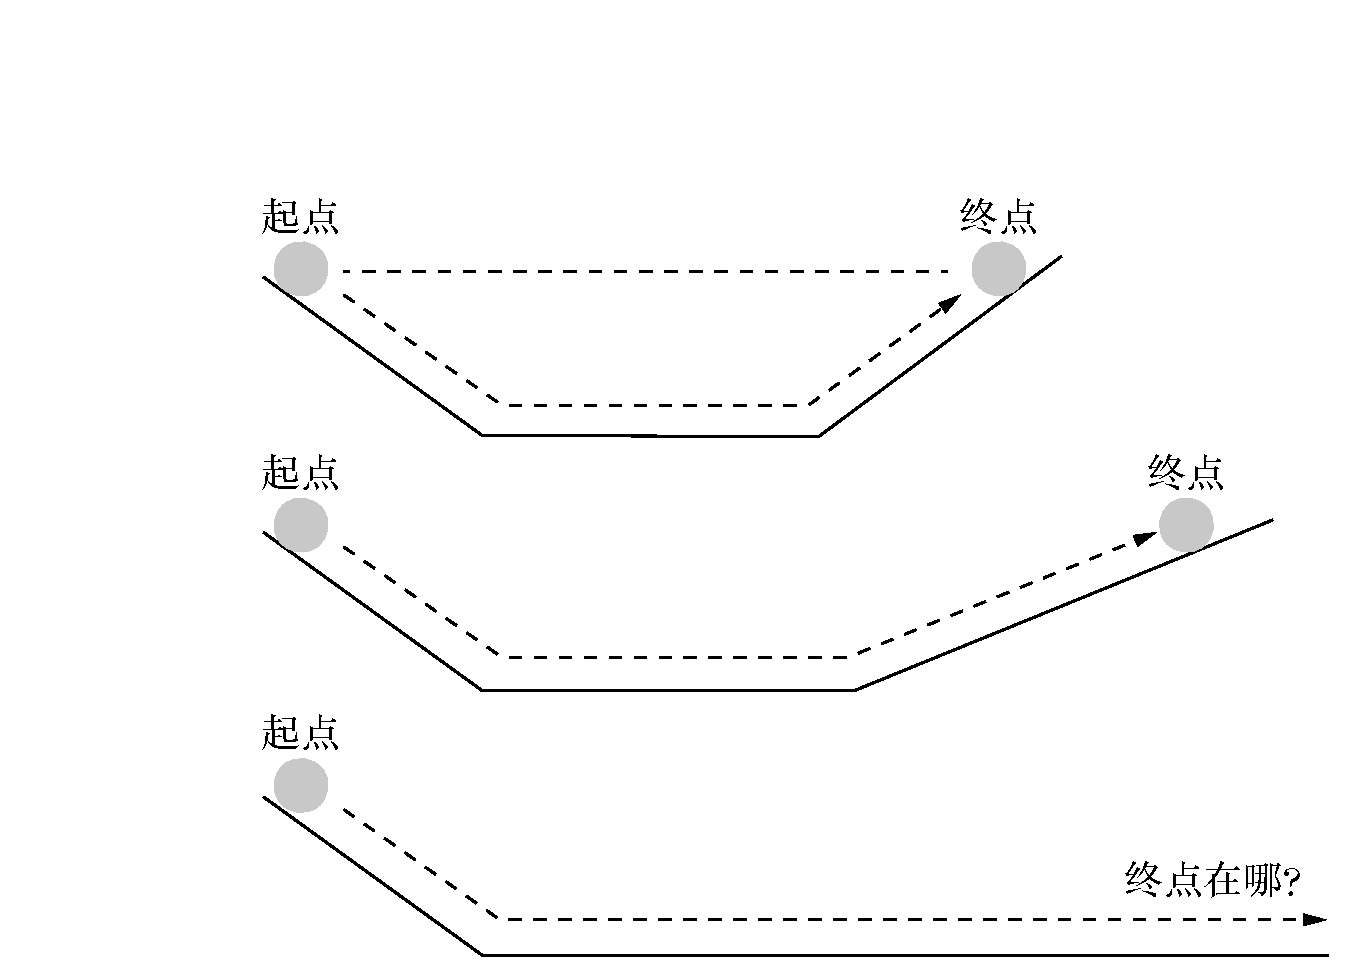
\includegraphics{Galileo}
    \caption{Galileo斜面实验}
    \labfig{Galileo_slope_experiment}
\end{marginfigure}

这个误差就是上面提到的单元内误差.这种误差在是心理学中的一种非常特殊的误差,在物理实验中就不存在这样误差,比如在Galileo的斜面实验(slope experiment),可以看到\reffig{Galileo_slope_experiment}中每个圆球都会上升到同一个高度,不同的球在各种属性上都是完全相同的,所以重复实验对物理属性匹配了的圆球就会有相同效果.但是对于人而言,每个人都不一样,都带着性别、性格、年龄、教育程度等进入实验室,而这些因素会影响行为,我们无法做到匹配完全相同的两个人.
这个变异在完全随机设计中给我们提供了一个随机误差的估计,所有的处理效应都是和它相比,尽管这部分变异不完全是随机的,不过对于完全随机设计而言已经没有更好的办法了.

从这个角度上来说,任何实验中每一组内都不可能只用一个被试,如果只有一个被试就没有变异了,起码两个人才有变异.

\subsection{评价}

完全随机实验设计的\textbf{优点}是,实验设计和实施简单,接受每个处理水平的被试数量可以不相等,不需要匹配被试,每个被试公接受一个处理水平.完全随机实验的统计分析和对结果的解释简单,并且与它的误差平方和相对应的自由度最大。因此,如果在不同的实验设计中得到的误差平方和相等,那么完全随机实验设计比其他实验设计更敏感.

完全随机实验设计的\textbf{缺点}是,它的组内变异并非全部由随机误差组成,其中还包括了被试的个体差异.虽然完全随机设计假设随机分配的各组被试在统计上是无差异的,但实际上被试的个体差异带来的无关变异是存在的,并且混杂在组内变异中,导致$F$比率的分母项加大, 从而使实验较为不敏感.另外,当实验中含多个处理水平时,需要的被试量也会较大.